\documentclass[border=4pt]{standalone}
\usepackage{amsmath}
\usepackage{tikz}
\usetikzlibrary{arrows}
\begin{document}
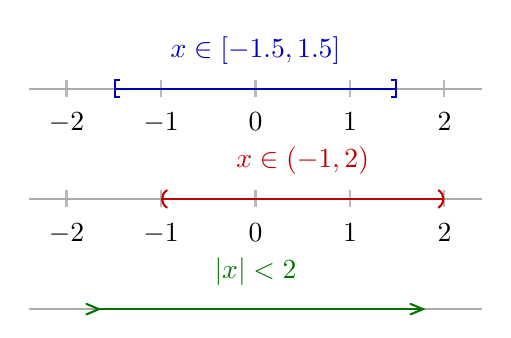
\begin{tikzpicture}[x=12mm,y=9mm,line width=.75pt]
  \foreach \x in {-2,-1,0,1,2} {
    \draw[gray!55] (\x,-.12) -- (\x,.12);
    \node[below=2pt] at (\x,-.12) {$\x$};
  }
  \draw[gray!65] (-2.4,0) -- (2.4,0);
  \draw[blue!75!black,{square bracket}-{square bracket}] (-1.5,0) -- (1.5,0);
  \node[above=5pt,blue!75!black] at (0,0) {$x\in[-1.5,1.5]$};

  \begin{scope}[yshift=-14mm]
    \foreach \x in {-2,-1,0,1,2} {
      \draw[gray!55] (\x,-.12) -- (\x,.12);
      \node[below=2pt] at (\x,-.12) {$\x$};
    }
    \draw[gray!65] (-2.4,0) -- (2.4,0);
    \draw[red!75!black,{(}-{)}] (-1,0) -- (2,0);
    \node[above=5pt,red!75!black] at (.5,0) {$x\in(-1,2)$};
  \end{scope}

  \begin{scope}[yshift=-28mm]
    \draw[gray!65] (-2.4,0) -- (2.4,0);
    \draw[green!45!black,{angle 45 reversed}-{angle 45}] (-1.8,0) -- (1.8,0);
    \node[above=5pt,green!45!black] at (0,0) {$|x|<2$};
  \end{scope}
\end{tikzpicture}
\end{document}
